% THIS IS AN EXAMPLE DOCUMENT FOR VLDB 2012
% based on ACM SIGPROC-SP.TEX VERSION 2.7
% Modified by  Gerald Weber <gerald@cs.auckland.ac.nz>
% Removed the requirement to include *bbl file in here. (AhmetSacan, Sep2012)
% Fixed the equation on page 3 to prevent line overflow. (AhmetSacan, Sep2012)

\documentclass{vldb}
\usepackage{graphicx}
\usepackage{hyperref}
\usepackage{gensymb}
\usepackage{textcomp}
\usepackage{siunitx}

\usepackage[bottom]{footmisc}

\usepackage{balance}  % for  \balance command ON LAST PAGE  (only there!)
\graphicspath{{images/}} 

\begin{document}

% ****************** TITLE ****************************************

\title{Global Warming Distributed Data Analysis}

% possible, but not really needed or used for PVLDB:
%\subtitle{[Extended Abstract]
%\titlenote{A full version of this paper is available as\textit{Author's Guide to Preparing ACM SIG Proceedings Using \LaTeX$2_\epsilon$\ and BibTeX} at \texttt{www.acm.org/eaddress.htm}}}

% ****************** AUTHORS **************************************

% You need the command \numberofauthors to handle the 'placement
% and alignment' of the authors beneath the title.
%
% For aesthetic reasons, we recommend 'three authors at a time'
% i.e. three 'name/affiliation blocks' be placed beneath the title.
%
% NOTE: You are NOT restricted in how many 'rows' of
% "name/affiliations" may appear. We just ask that you restrict
% the number of 'columns' to three.
%
% Because of the available 'opening page real-estate'
% we ask you to refrain from putting more than six authors
% (two rows with three columns) beneath the article title.
% More than six makes the first-page appear very cluttered indeed.
%
% Use the \alignauthor commands to handle the names
% and affiliations for an 'aesthetic maximum' of six authors.
% Add names, affiliations, addresses for
% the seventh etc. author(s) as the argument for the
% \additionalauthors command.
% These 'additional authors' will be output/set for you
% without further effort on your part as the last section in
% the body of your article BEFORE References or any Appendices.

\numberofauthors{2} %  in this sample file, there are a *total*
% of EIGHT authors. SIX appear on the 'first-page' (for formatting
% reasons) and the remaining two appear in the \additionalauthors section.

\author{
% You can go ahead and credit any number of authors here,
% e.g. one 'row of three' or two rows (consisting of one row of three
% and a second row of one, two or three).
%
% The command \alignauthor (no curly braces needed) should
% precede each author name, affiliation/snail-mail address and
% e-mail address. Additionally, tag each line of
% affiliation/address with \affaddr, and tag the
% e-mail address with \email.
%
% 1st. author
\alignauthor Alberto Simioni\\
       \affaddr{number}\\
       \email{mail}
% 2nd. author
\alignauthor Federico Ziliotto\\
       \affaddr{2577394}\\
       \email{f.z.ziliotto@student.vu.nl}
}
\date{}


\maketitle

\begin{abstract}


\end{abstract}

\section{Introduction}
\label{sec:intro}
Global warming is an open topic of discussion today. While climate scientist debate on the causes of the gradual temperature rise in the past 50 years (the majority claim the increase of CO2 due to fossil fuel is to blame, other researchers found alternative explanations, like non CO2 greenhouse gases (GHGs) \cite{hansen2000global}), data scientist had access to ever increasing technologies and data sources to study the phenomenon. Whatever the causes, the data collected by different organizations and from different parts of the world all agree that the global temperature in the world is rising \cite{hansen2006global}. We show that this trend is not only real, but the temperature increase is accelerating in the last twenty years at a worrisome rate. We aim to update the results obtained by other institutions with the more recent data, and to do that we want to use more flexible and powerful tools. With the use of distributed computing technologies (like the Hadoop file system and the Spark programming framework) we want to show the capabilities but also the limitations of this new technologies applied in large scale computing. Moreover, we created and interactive tool that may help researchers to visualize the enormous amount of climate data that was collected in the past century and detect possible global warming causes and effects.

\subsection{Data Sources}
We have access to more than one hundred years of weather data provided by the NOAA (National Oceanic and Atmospheric Administration) organization. The raw data is publicly accessible\footnote{\href{ftp://ftp.ncdc.noaa.gov/pub/data/noaa/}{Noaa public data}}, so anyone interested in analyzing the climate of the past years can use them. The data is organized by year and grouped by ISD (Integrated Surface Data) stations. They also provide a \texttt{perl} script that helps in reading and viewing the data. NOAA also publishes monthly reports on the climate status (like temperature, precipitation, sea level) and compares the data obtained for the last month/year to the averages calculated in the past, accompanied by a software suite to repeat or modify the analysis at home. While this tools and datasets are helpful, there are currently no publicly available tools to perform custom data analysis on the whole raw dataset available. In particular, considering the size of the uncompressed data (\~205 GB) it may be necessary to use a cluster to make complex computations that require more time. 

\subsection{Our Contribution}
Our aim is to update the recent work done in the climate analysis with the new data available. Moreover we will perform the analysis in a cluster and study a way to improve the analysis performance in this type of environment. In the end, we will compare the results we obtained with the ones available in the literature and evaluate the state of global warming in the recent years.\\

In the following sections we first describe the context of our work and the related literature in section \ref{sec:rel}, then we explain how we implemented the data analysis in section \ref{sec:pro}, then we describe the analysis (\ref{sec:exp}). In section \ref{sec:res} we show the results we obtained and discuss them and finally in section \ref{sec:con} we argue the relevance of our results and future improvements.


\section{Related Work}
\label{sec:rel}
Studies on global and regional surface temperature change has been done in past. Researchers showed that the rate of temperature increase has been higher in the last quarter of the century that it has been in the previous years of the 20\^{th} century. Moreover they calculated an increase in the average global five year mean of about 1\celsius~\cite{hansen1999giss}. This recent trend is particularly important if we consider the temperature changes in the past millennium, and can be considered an unprecedented anomaly\cite{mann1999northern}. More recent studies also show that the mean annual temperature has not risen in the last twenty years, despite the continuous increase of GHGs in the atmosphere\cite{kosaka2013recent}. This suggests that either the global warming phenomenon that was registered in the period 1975-2000 had different causes or that the more recent stable trend has an origin that balance the greenhouse effects.

\section{Research Question}



\section{Project setup}
\label{sec:pro}
In this section we explain in more detail how we performed the analysis, what tools we used and the preliminary work on the data before the analysis. 


\subsection{Data Format}
The public NOAA data repository contains a file for each station for each year. The name of each file is \{USAF code\}\-\{WBAN code\}-\{year\}, where USAF is the Air Force Station ID and the WBAN is the NCDC (National Climate Data Center) station number. The number of station for each year is shown in figure \ref{fig:stations}. As we can see the number of stations has steadily increased during the years. More importantly, we have to be aware of the results we obtain analyzing years where the number of stations is very low. Since the distribution of the station around the world is not uniform and they don't cover every area, it's difficult to obtain correct results on the global scale. What we can do is to consider the fluctuation of data for the same station or for stations that are near together (this will be done by regional grouping, as described in section \ref{sec:pro}). Each station report data multiple times a day (depending on the station) and for each day of the year. \\

\begin{figure}[tbh]
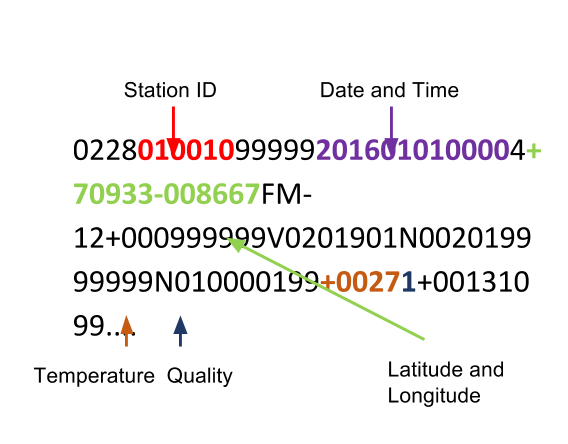
\includegraphics[width=1\linewidth]{data}
\caption{Measurement format}
\label{fig:data}
\end{figure}

Each measurement comes in a form similar to what \ref{fig:data} shows. The information we need for our analysis are: station ID, data and time, coordinates (in latitude and longitude), the temperature value and the quality of the temperature measurement.


\subsection{Temperature data quality}
\label{sec:filter}
Before using the actual temperature data, we filtered it through a custom quality check. Each measurement come with a quality flag set at a different value depending on how reliable the measurement was\cite{noaaDataFormat}. In particular we accepted all the measurement with the following quality code value:
\begin{itemize}
    \item 0: Passed gross limits check;
    \item 1: Passed all quality control checks;
    \item 4: Passed gross limits check, data originate from an NCEI data source;
    \item 5: Passed all quality control checks, data originate from an NCEI data source;
    \item A: Data value flagged as suspect, but accepted as a good value;
    \item I: Data value not originally in data, but inserted by validator;
    \item M: Manual changes made to value based on information provided by NWS or FAA;
    \item P: Data value not originally flagged as suspect, but replaced by validator;
    \item R: Data value replaced with value computed by NCEI software;
    \item U: Data value replaced with edited value.
\end{itemize}
We opted for a loose policy on the data quality, accepting also values that didn't pass all the quality checks or that were manually or software replaced. We refuted all the codes that stand for erroneous, missing or suspect data that was not manually or automatically checked and replaced by the institution. Furthermore, we applied a bound check for all the values greater than the maximum registered temperature (+61.8 \celsius) and the minimum one (-93.2 \celsius). \\
The data collected can be of two different types depending on the origin: from a fixed weather station or from a mobile one. In the second case, it's possible that the data registered from a mobile station (e.g. on a ship) is reported at a certain position and the following measurement is reported at a different position. Since we didn't distinguish data by time of the day, it's important that the number of measurements from a certain position is approximately the same for different hours. Since this is not guaranteed by moving stations, we decided to filter the measurement obtained from this source. \\

\subsection{Data Sources}
An important aspect we had to consider before proceeding with the analysis is the distribution of weather station on the globe. First we considered the number of stations per year\ref{fig:stations}. Then we analyzed the position of the stations for each year (some notable sample are reported in appendix \ref{App:AppendixA}). 

\begin{figure}[tbh]
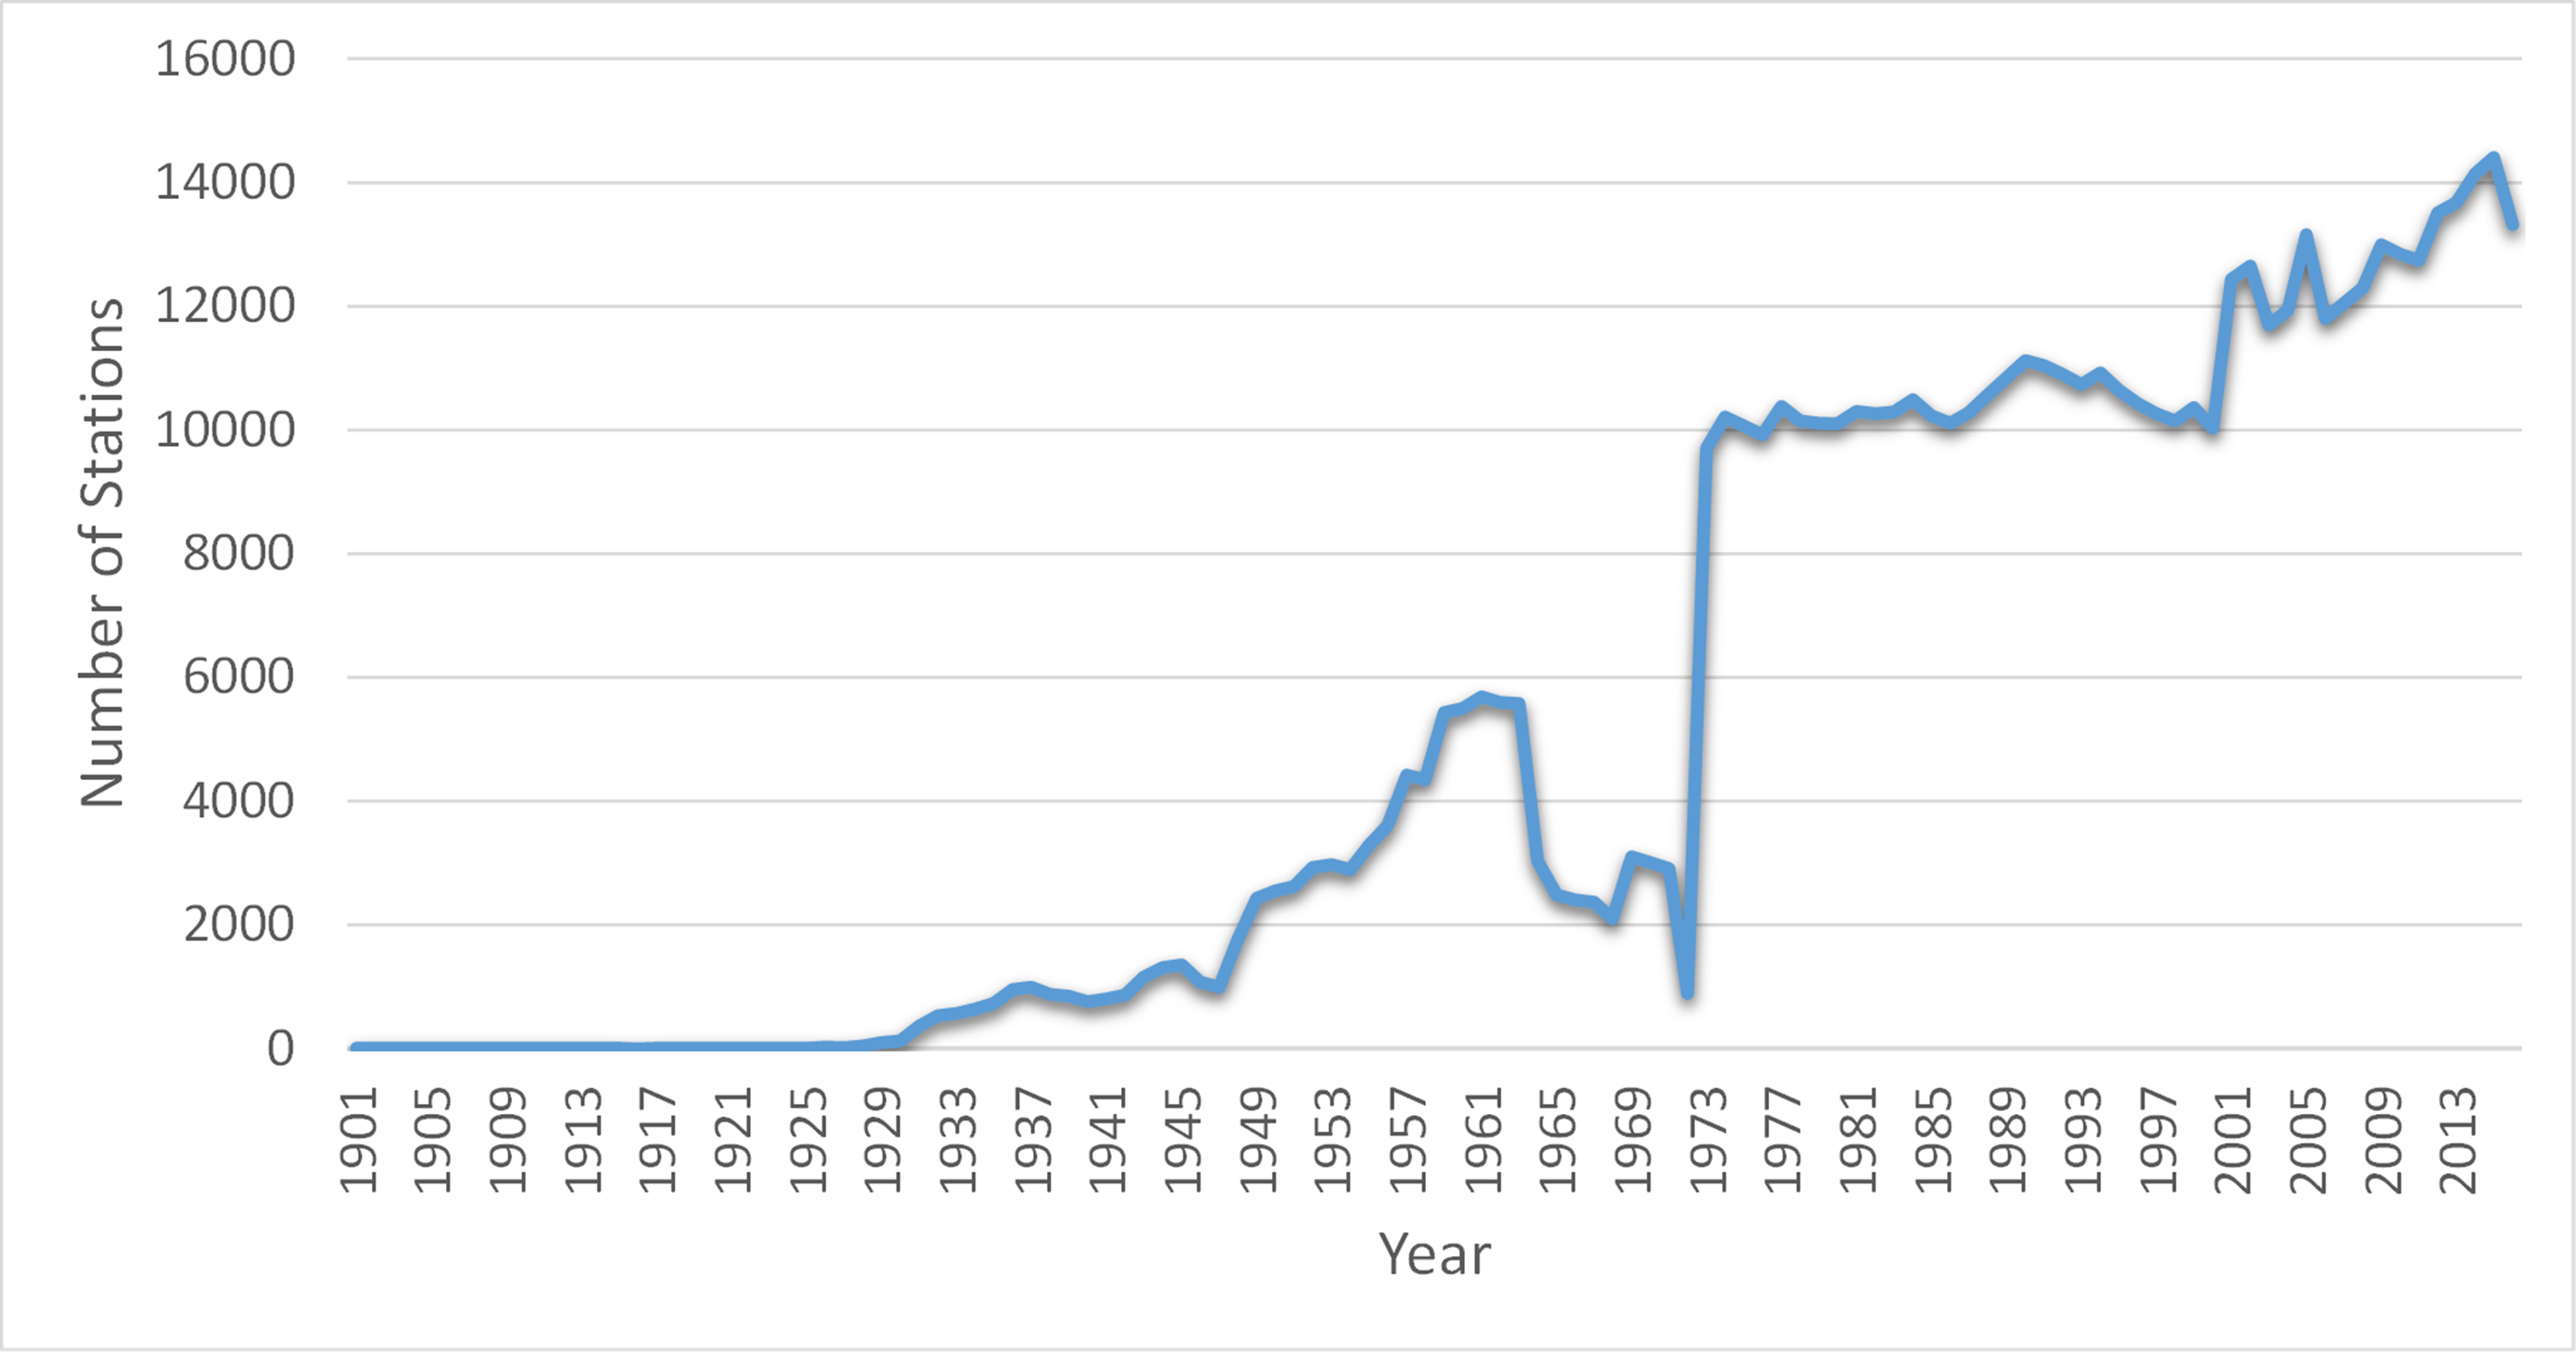
\includegraphics[width=1\linewidth]{stations}
\caption{Number of stations per year}
\label{fig:stations}
\end{figure}

Considering that the stations for most of the years are not uniformly distributed, we decided to take analyze the global temperature averages only for some selected regions that have the highest amount of data available (e.g. the United States and European area). \\
Nonetheless, we calculated for each year the mean, minimum and maximum temperature


\subsection{Distributed environment}
The technological environment we decided to use for this project consist of:

\textbf{HDFS}\footnote{\url[Hadoop Distributed File System]{http://hadoop.apache.org/}}: a distributed file system that allows the developers to store and retrieve large quantity of data between multiple machines as if it was a single one;
\textbf{Spark}\footnote{\url[Apache Spark]{http://spark.apache.org/}}: programming framework to develop applications for large scale data processing on horizontally scalable clusters. The choice of this technology is motivated by size of the data and the type of the analysis we want to execute. First, Spark is more efficient than Hadoop's own MapReduce\cite{dean2008mapreduce} implementation when the data used can fit in memory. Since our approach is to analyze one or a few years at a time, we calculated that the size of the data is small enough to stay in memory for our purposes. The second advantage is that we would like to make multiple transformations to the data and Spark allows to easily cache the intermediate results to be reused efficiently.\\

\begin{figure}[tbh]
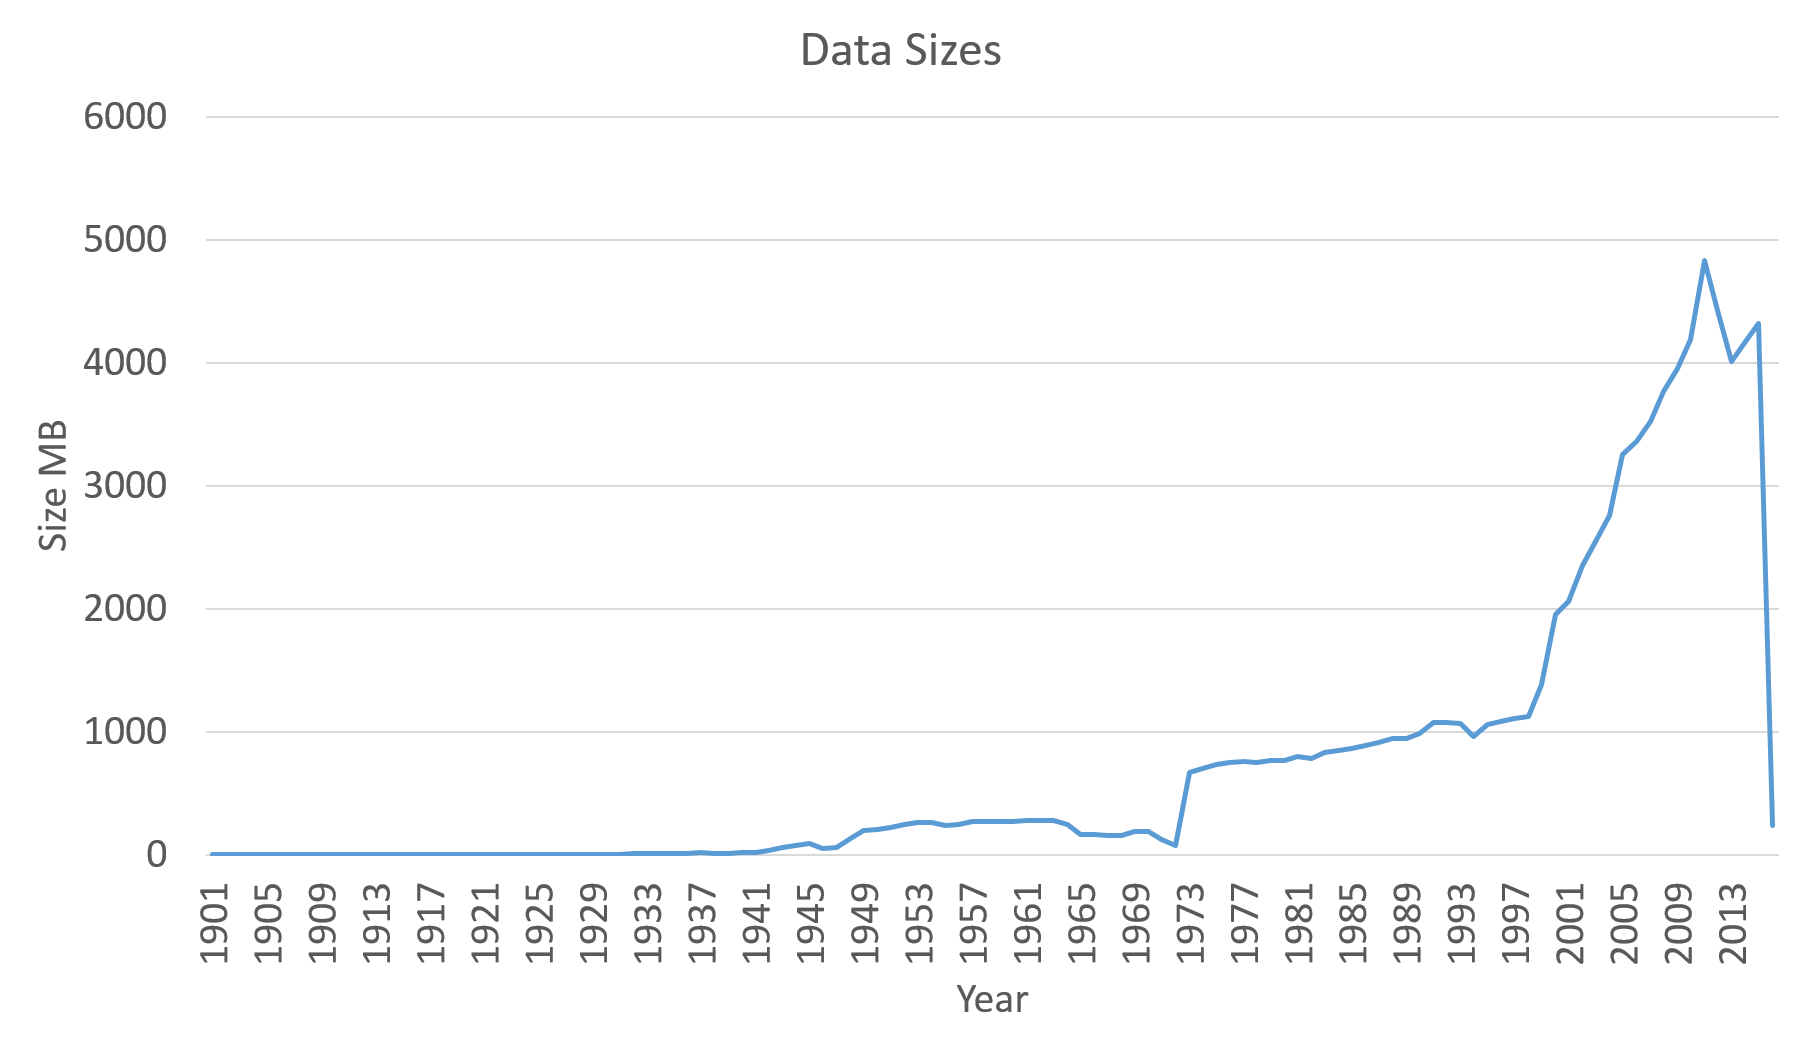
\includegraphics[width=1\linewidth]{dataSize}
\caption{Size of the data per year}
\label{fig:dataSize}
\end{figure}

The data stored in the distributed file system is grouped in folder by year. As shown in figure \ref{fig:dataSize} the size of the data to analyze is very different between the years. Inside each folder, there is a file for each station that reported measurements. HDFS is not very efficient when working with many small files\cite{zhang2012improving}, as in our case. The solution we opted to use is to merge the small files in bigger files that have the same size as Hadoop's default block size. To merge the files we used is filecrusher\footnote{\url[Hadoop Filecrusher]{https://github.com/edwardcapriolo/filecrush}}. \\


\subsection{Analysis Tools}
In this section we briefly present the programming environment we use and the algorithm we implemented to analyze the NOAA dataset.


\section{Experiments}
\label{sec:exp}
We performed two main type of analysis: a five year span analysis that considers all the measurement reported by stations near each other in five years, and an analysis on large earth regions on a yearly basis. \\
The basic steps that both analysis perform are:
\begin{enumerate}
    \item Load data in memory;
    \item Parse the raw data to obtain an list of StationData (a type that represent a measurement);
    \item Filter data following the scheme indicated in \ref{sec:filter};
    \item Group the measurements in regions
    \item Execute analysis;
    \item Save results;
\end{enumerate}

\subsection{Regional five year period analysis}
The aim of this analysis is to calculate the temperature statistics (mean, maximum and minimum) on every area of the earth for which we have data. After that we can compare the situation for the same areas in different time frames and show it with a world map view (as shown in \ref{sec:map}). \\
The first problem is that while the regions we want to compare are the same size and uniformly distributed around the earth, the stations are not. So we defined regions of size 1\degree latitude and 1\degree longitude. This is approximately the area covered by the region of Holland in the Netherlands. Then we assigned each measurement (for each one there is the coordinates reported) to a region. \\
Our analysis proceeded by loading five consecutive years of measurements at a time, group them in small regions and, for each region, calculate the arithmetic mean, the minimum and the maximum temperature. This was done for all years from 1901 to 2015 (the year 2016 was excluded from the analysis due to incomplete data).\\


\subsection{Temperature yearly trends analysis}
In this type of analysis we focused on some particular large areas of on the earth. We selected the regions that for which we have more and better distributed data available. The selected regions are:
\begin{itemize}
    \item United States: from coordinate N\ang{50;;} W\ang{128;;} to N\ang{24;;} W\ang{65;;};
    \item Europe: from coordinate N\ang{71;;} W\ang{11;;} to N\ang{35;;} E\ang{41;;};
    \item Australia: from coordinate S\ang{9;;} E\ang{111;;} to S\ang{44;;} E\ang{156;;};
\end{itemize}
For each region we calculated average, minimum and maximum of every year from 1980 to 2015. The year range is chosen based on the availability of data.

\section{Results}
\label{sec:res}
In this section we report the results obtained from the analysis described in section \ref{sec:exp}. 

\section{Conclusions}
\label{sec:con}

\newpage
\appendix
\section{Stations distribution} \label{App:AppendixA}
Here is an overview of the stations for some selected years. We decided to show only years in which the number and position of the stations is significantly different than in the previous or following years.

\begin{figure}[tbh]
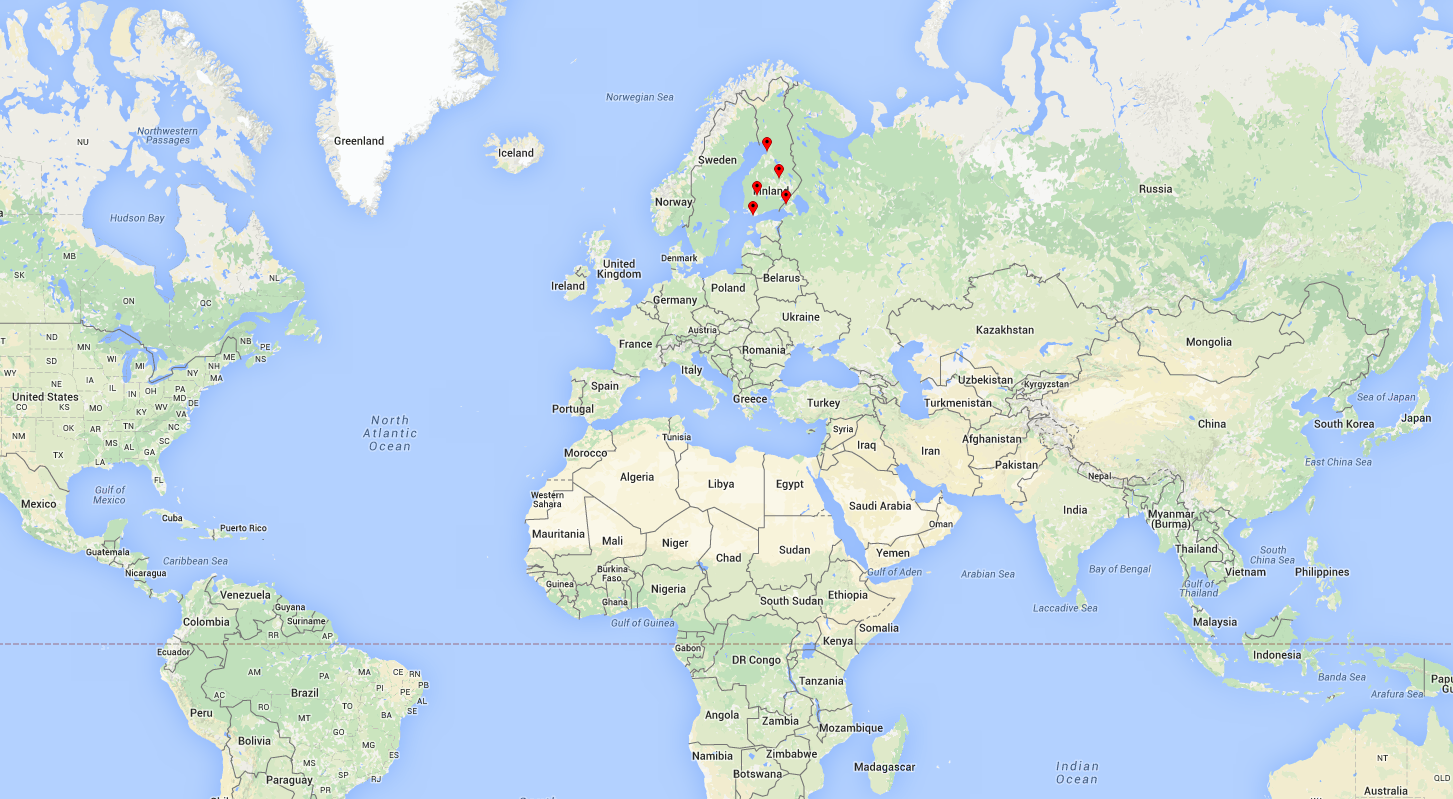
\includegraphics[width=1\linewidth]{stations1907}
\caption{In the first years we only have measurements coming from stations in Finland}
\label{fig:stations1907}
\end{figure}

\begin{figure}[tbh]
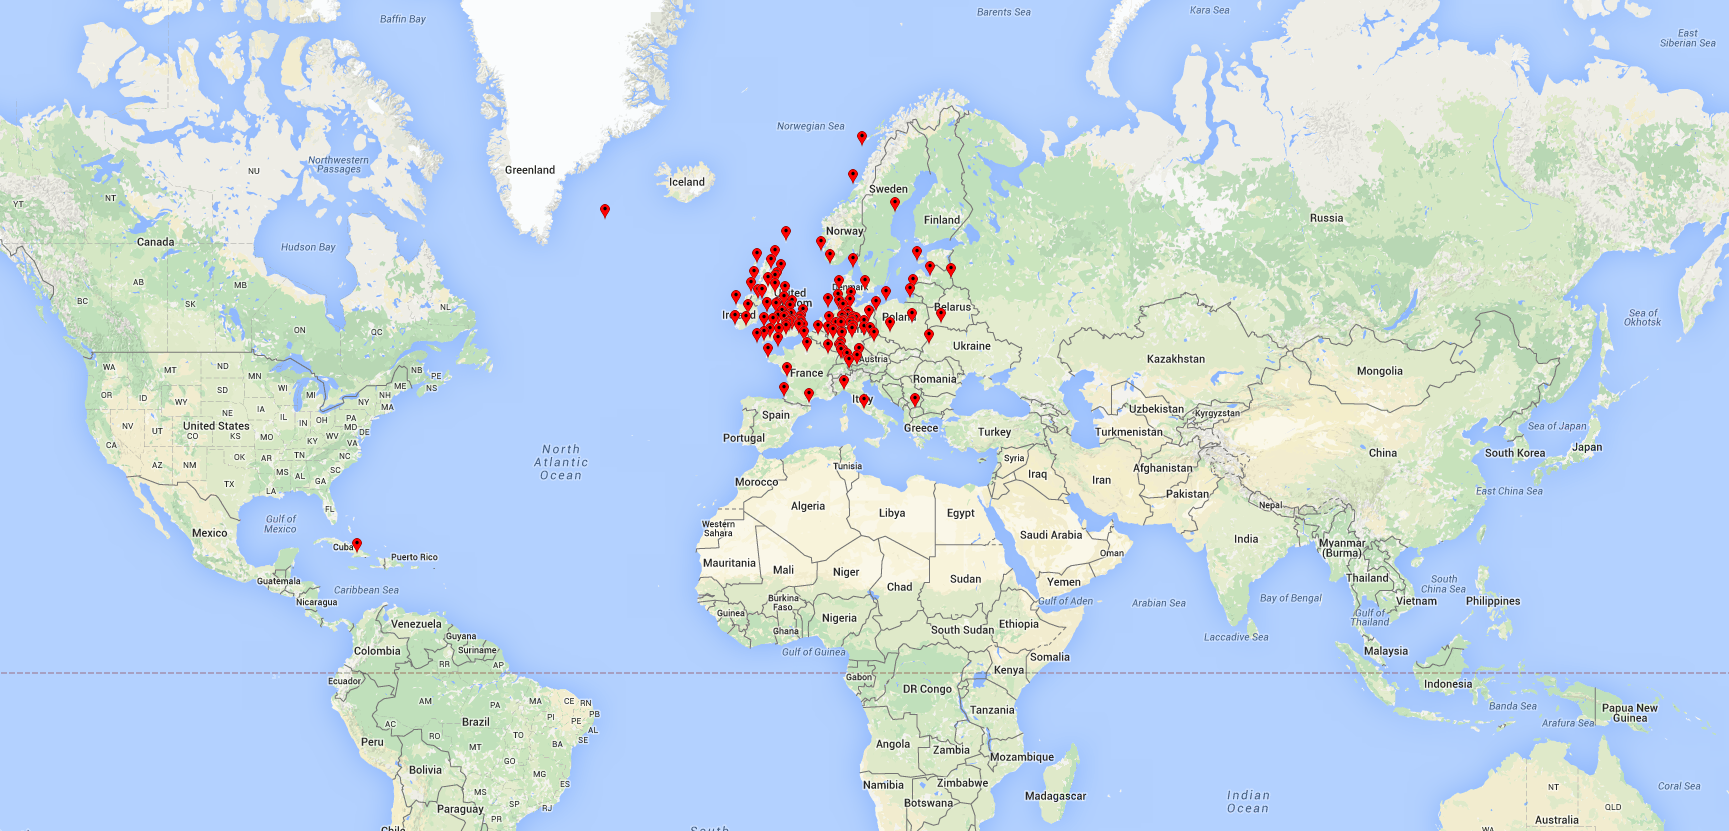
\includegraphics[width=1\linewidth]{stations1930}
\caption{Here we can see the stations cover the most part of central Europe. The problem we encountered is that there is no continuity in the stations that are used between consecutive years, so it's difficult to make comparisons.}
\label{fig:stations1930}
\end{figure}

\begin{figure}[tbh]
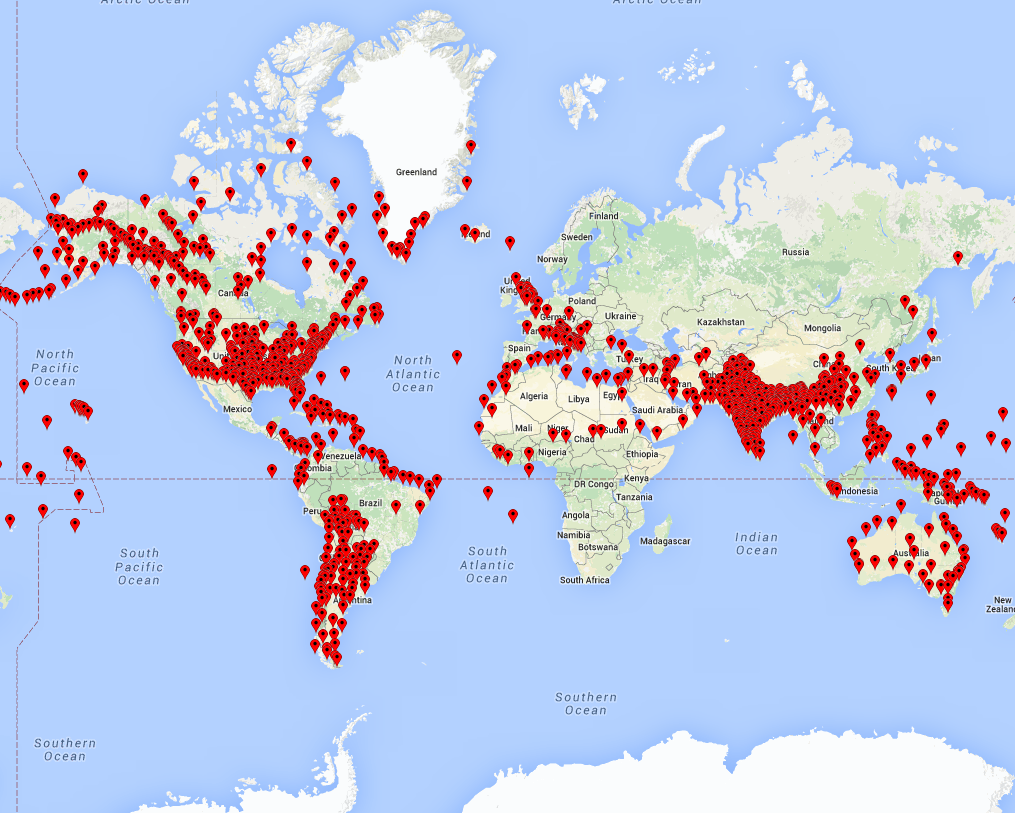
\includegraphics[width=1\linewidth]{stations1945}
\caption{Around this year we start to have a relevant number of stations that cover most part of the surface.}
\label{fig:stations1945}
\end{figure}

\begin{figure}[tbh]
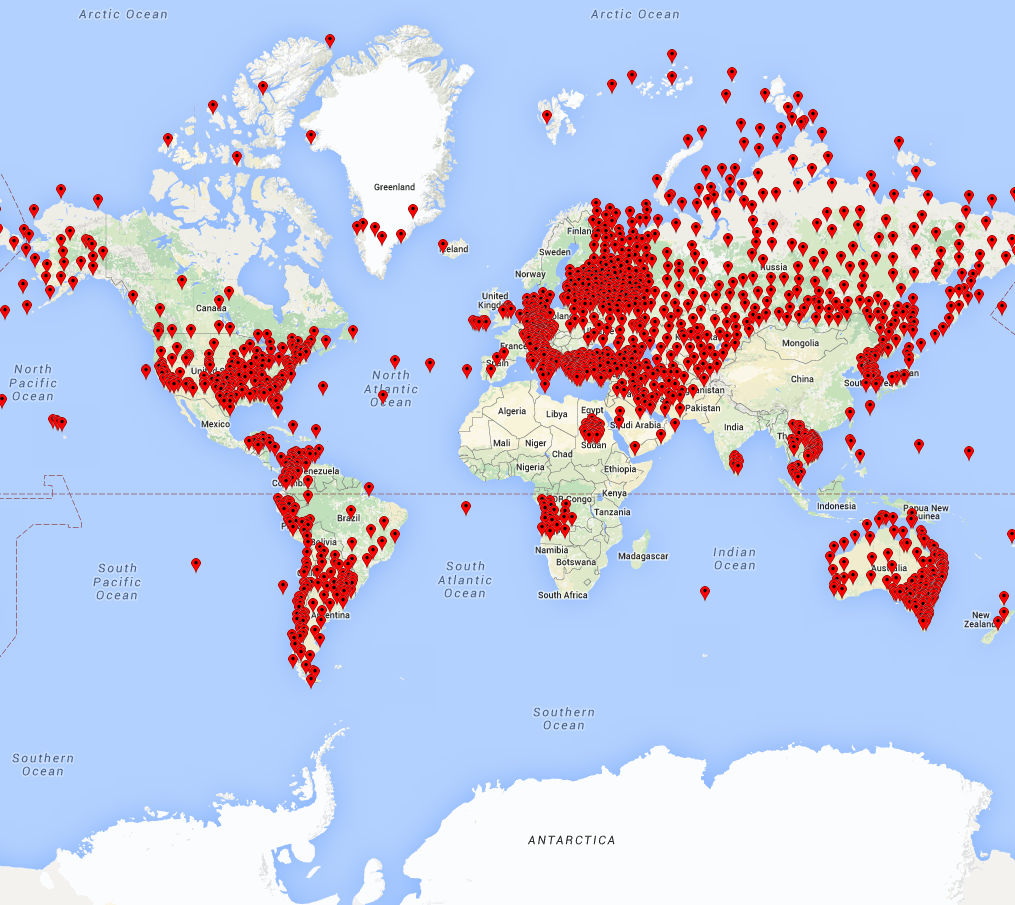
\includegraphics[width=1\linewidth]{stations1968}
\caption{In the late 60s we notice a sudden drop in the earth coverage compared to the previous years. We took this into account when making the analysis.}
\label{fig:stations1968}
\end{figure}

\begin{figure}[tbh]
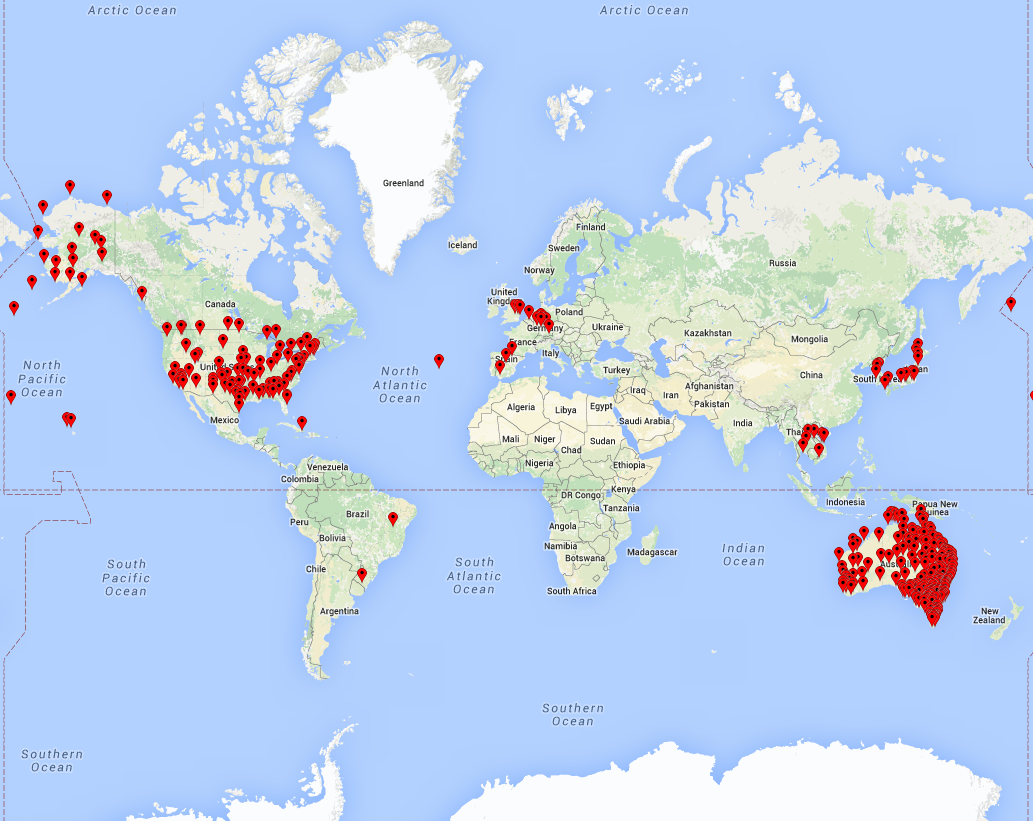
\includegraphics[width=1\linewidth]{stations1972}
\caption{As shown in figure \ref{fig:stations}, we noticed a sudden drop in the number of stations for this year. In particular we observe the absence of stations from east Europe and the ex Soviet Union Area.}
\label{fig:stations1972}
\end{figure}

\begin{figure}[tbh]
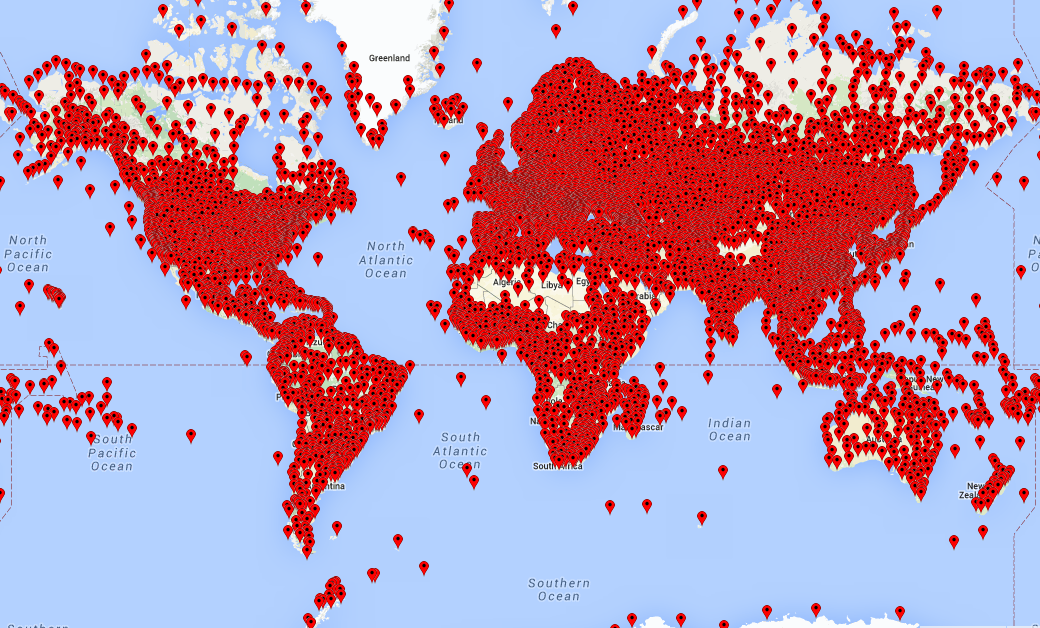
\includegraphics[width=1\linewidth]{stations1980}
\caption{From this year onwards we have a large number of stations covering most part of the surface.}
\label{fig:stations1980}
\end{figure}

\begin{figure}[tbh]
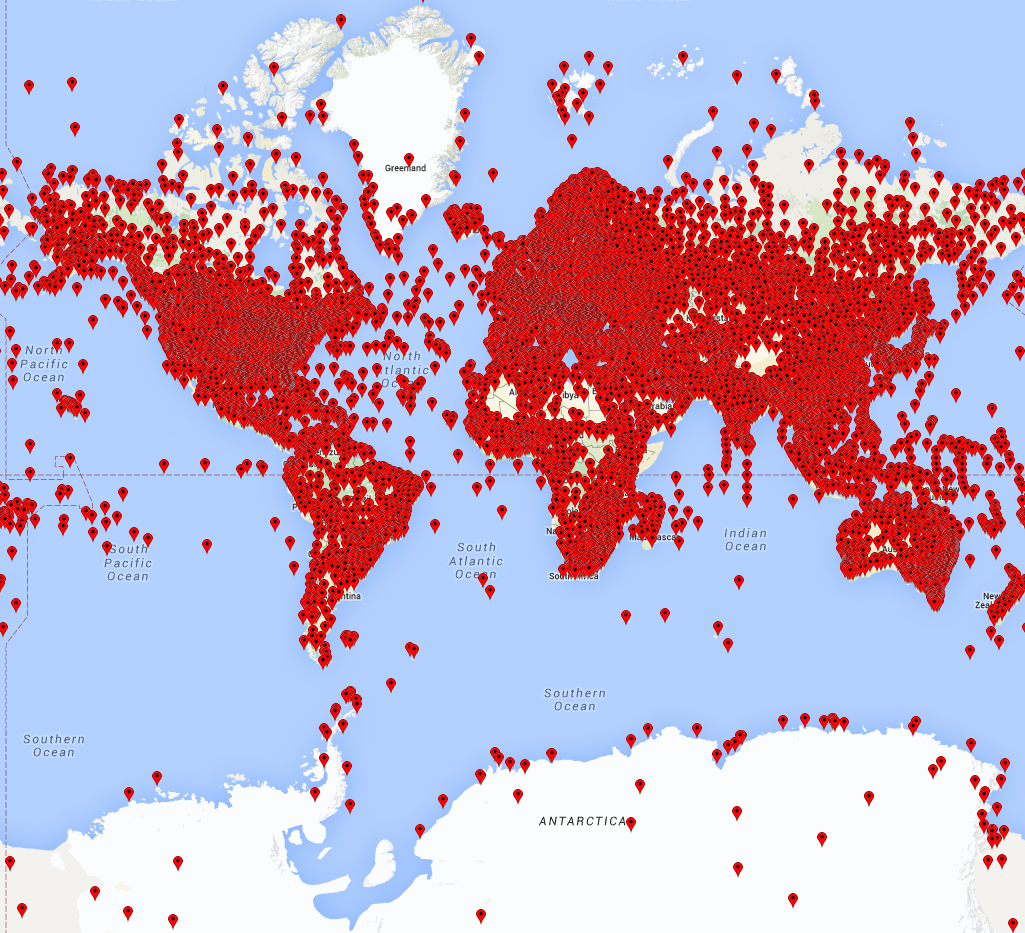
\includegraphics[width=1\linewidth]{stations2014}
\caption{Measurement format}
\label{fig:stations2014}
\end{figure}

\clearpage
%\end{document}  % This is where a 'short' article might terminate

% ensure same length columns on last page (might need two sub-sequent latex runs)
\balance

%ACKNOWLEDGMENTS are optional
%\section{Acknowledgments}


% The following two commands are all you need in the
% initial runs of your .tex file to
% produce the bibliography for the citations in your paper.
\bibliographystyle{ieeetr}
\bibliography{vldb_sample}  % vldb_sample.bib is the name of the Bibliography in this case
% You must have a proper ".bib" file
%  and remember to run:
% latex bibtex latex latex
% to resolve all references

%Generated by bibtex from your ~.bib file.  Run latex,
%then bibtex, then latex twice (to resolve references).




\end{document}
